\documentclass[a4paper,14pt]{article}
\usepackage{float}
\usepackage{extsizes}
\usepackage{amsmath}
\usepackage{amssymb}
\everymath{\displaystyle}
\usepackage{geometry}
\usepackage{fancyhdr}
\usepackage{multicol}
\usepackage{graphicx}
\usepackage[brazil]{babel}
\usepackage[shortlabels]{enumitem}
\usepackage{cancel}
\usepackage{textcomp}
\columnsep=2cm
\hoffset=0cm
\textwidth=8cm
\setlength{\columnseprule}{.1pt}
\setlength{\columnsep}{2cm}
\renewcommand{\headrulewidth}{0pt}
\geometry{top=1in, bottom=1in, left=0.7in, right=0.5in}

\pagestyle{fancy}
\fancyhf{}
\fancyfoot[C]{\thepage}

\begin{document}
	
	\noindent\textbf{8FMA71 - Matemática} 
	
	\begin{center}Gráficos de relações dadas por uma equação de duas variáveis (Versão estudante)
	\end{center}
	
	\noindent\textbf{Nome:} \underline{\hspace{10cm}}
	\noindent\textbf{Data:} \underline{\hspace{4cm}}
	
	%\section*{Questões de Matemática}
	
	
    \begin{multicols}{2}
    	\noindent Para esboçarmos o gráfico de uma relação podemos determinar as coordenadas de alguns pontos através da tabela
    	\noindent\textsubscript{~---------------------------------------------------------------------------}
		\begin{enumerate}
			\item Esboçar, determinando no mínimo 5 pontos distintos, os gráficos das seguintes relações:
			\begin{enumerate}[a)]
				\item $y = x^3$ \\\\\\\\\\\\\\\\\\\\\\\\\\\\
				\item $x = y^2$ \\\\\\\\\\\\\\\\\\
			\end{enumerate}
		    \item Faça os gráficos das seguintes relações:
		    \begin{enumerate}[a)]
		    	\item $(x - 2)(y + 4) = 0$ \\\\\\\\\\\\\\\\\\\\\\\\\\\\
		    	\item $x^2 = y^2$ \\\\\\\\\\\\\\\\\\\\\\\\\\\\\\\\
		    \end{enumerate}
	        \item Determine os valores das constantes $a$, $b$ e $c$ para que $y = ax^2 + bx + c$ tenha como gráfico:
	        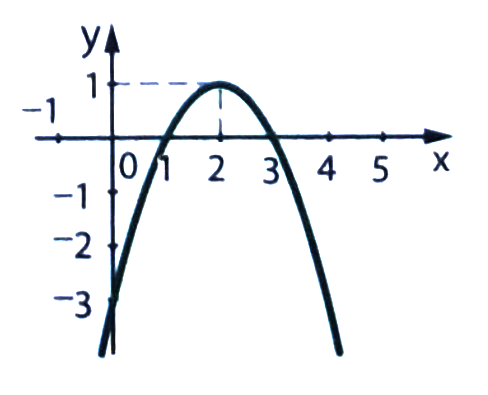
\includegraphics[width=1\linewidth]{imagens_8FMA71/imagem1} \\\\\\\\\\\\\\\\\\\\\\\\\\\\\\\\\\\\\\\\\\\\\\\\\\\\\\
	        \item Esboce os gráficos das relações a seguir, determinando no mínimo quatro pontos distintos. 
	        \begin{enumerate}[a)]
	        	\item $y = x$ \\\\\\\\\\\\\\\\\\\\\\\\\\\\\\\\\\\\
	        	\item $y = \frac{8}{x}, x \in \mathbb{R_+^*}$ \\\\\\\\\\\\\\\\\\\\\\\\\\\\\\\\\\
	        	\item $y = -x^2 + 6$ \\\\\\\\\\\\\\\\\\\\\\\\\\\\
	        	\item $y = |x|$ \\\\\\\\\\\\\\\\\\\\\\\\\\\\
	        \end{enumerate}
            \item Com base no gráfico da relação $y = 3^x$, analise as afirmações a seguir e classifique-as em \textbf{V} (verdadeiro) ou \textbf{F} (falso).
            \begin{enumerate}[a)]
            	\item (~~) O gráfico intersecta o eixo das abscissas.
            	\item (~~) A abscissa não pode assumir valores negativos.
            	\item (~~) O gráfico se encontra totalmente acima do eixo das abscissas.
            	\item (~~) O gráfico cruza o eixo das ordenadas no ponto (0; 1).
            	\item O gráfico da relação é:
            	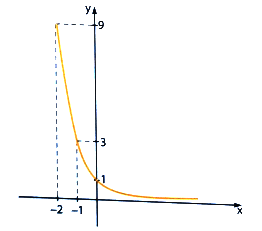
\includegraphics[width=1\linewidth]{imagens_8FMA71/imagem2}
            \end{enumerate}
        	\item Determine os valores das constantes $a$ e $b$, ára que o gráfico da relação $(x - a) \cdot (y - b) = 0$ passe pelo ponto (2; -3). \\\\\\\\\\\\\\\\\\\\\\\\\\\\\\\\\\\\\\\\
        	\item Determine os valores das constantes $a, b$ e $c$, com $c > 0$, para que a relação $y = \frac{ax + b}{c^x}$ tenha como gráfico:
        	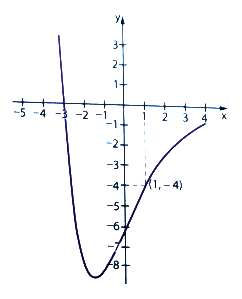
\includegraphics[width=1\linewidth]{imagens_8FMA71/imagem3}
        \end{enumerate}
    $~$ \\ $~$ \\ $~$ \\ $~$ \\ $~$ \\ $~$ \\ $~$ \\ $~$ \\ $~$ \\ $~$ \\ $~$ \\ $~$ \\ $~$ \\ $~$ \\ $~$ \\ $~$ \\ $~$ \\ $~$ \\ $~$ \\ $~$ \\ $~$ \\ $~$ \\ $~$ \\ $~$ \\ $~$ \\ $~$ \\ $~$ \\ $~$ \\ $~$ \\ $~$ \\ $~$ \\ $~$ \\ $~$ \\ $~$ \\ $~$ \\ $~$ \\ $~$ \\ $~$ \\ $~$ \\ $~$ \\ $~$ \\ $~$ \\ $~$ \\ $~$ \\ $~$ \\ $~$ \\ $~$ \\ $~$ \\ $~$ \\ $~$ \\ $~$ \\ $~$ \\ $~$ \\ $~$ \\ $~$ \\ $~$ \\ $~$ \\ $~$ \\ $~$ \\ $~$ \\ $~$ \\ $~$ \\ $~$ \\ $~$
    \end{multicols}
\end{document}